%!TEX root = ../main.tex
\setcounter{chapter}{7}
\setcounter{section}{0}
\section{Digitization}
\vspace{-8pt} \hrule \hrule \hrule \hrule \hrule  \vspace{12pt}

$\bigstar$ Unit step function
\begin{align*}
	1_k(t) = \frac{1}{1+e^{-2kt}}&&&& 1(t) = \begin{cases}1 & t \geq 0 \\0 & t< 0\end{cases}\\
	1(t) = \lim_{k \rightarrow \infty} 1_k(t) 
\end{align*}


	    \begin{figure}[!h]
	        \centering
	        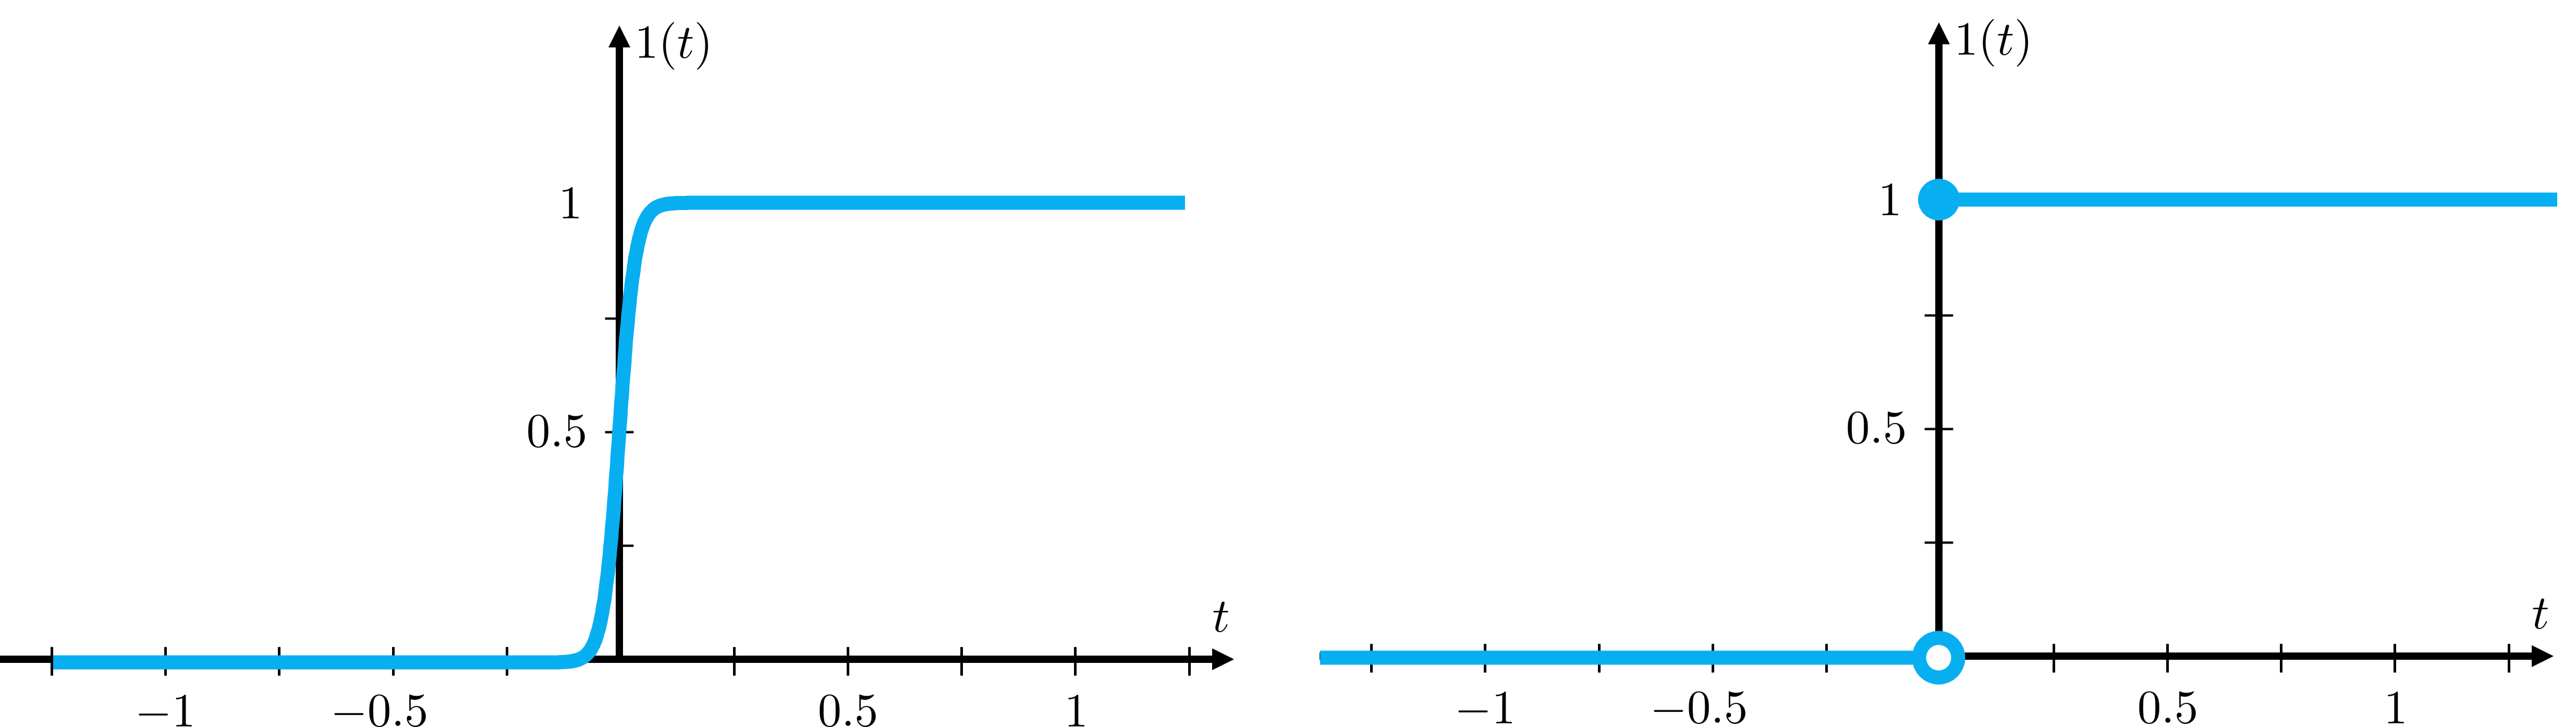
\includegraphics[width=18cm]{./FIG_Franklin/fig8-smc2_2.png}
	    \end{figure}


$\bigstar$ Useful Properties
 \begin{enumerate}
 	\item $\frac{d1(t)}{dt} = \delta(t) $ (수학적으로는 틀림, 개념적으로 사용)
 	\item $x(t)\delta(t-kT) = x(kT)\delta(t-kT)$
 	\item $\int_{-\infty}^{\infty} x(t) \delta(t-kT) dt= x(kT)$\\
		$ \because \int_{-\infty}^{\infty} x(t) \delta(t-kT)dt =\int_{-\infty}^{\infty} x(kT) \delta(t-kT) dt=x(kT)\int_{-\infty}^{\infty} \delta(t-kT) dt=x(kT)$
 	
 
 \end{enumerate}


